\documentclass[aspectratio=1610]{beamer}
\usetheme{bjeldbak}
\usepackage{xspace}
\usepackage{graphicx}
\usepackage{textpos}
\usepackage{subfigure}
\usepackage{pifont}
\usepackage[super]{nth}
\usepackage{relsize}
\usepackage{amsmath}

\setbeamertemplate{section page}{
  \begin{centering}
    \begin{beamercolorbox}[sep=12pt,center]{part title}
      \huge
      \insertsection
    \end{beamercolorbox}
  \end{centering}
}

\definecolor{anti-flashwhite}{rgb}{0.95, 0.95, 0.96}

\setbeamercolor{section in toc}{fg=anti-flashwhite}

\setbeamertemplate{section page}{
  \begin{centering}
    \begin{beamercolorbox}[sep=12pt,center]{part title}
      \huge
      \insertsection
    \end{beamercolorbox}
  \end{centering}
}

\usepackage{ifthen}
\usepackage{mciteplus} 
\newboolean{uprightparticles}
\setboolean{uprightparticles}{false} %Set true for upright particle symbols
\usepackage{xspace} 
\usepackage{upgreek}

\input{lhcb-symbols-def}
\input{spd-symbols-def}

\def \Cseven {\ensuremath{\mathcal{C}_{7}^{(\ensuremath{\prime})}}\xspace}
\def \Cnine {\ensuremath{\mathcal{C}_{9}^{(\ensuremath{\prime})}}\xspace}
\def \Cten {\ensuremath{\mathcal{C}_{10}^{(\ensuremath{\prime})}}\xspace}
\def \Cnineten {\ensuremath{\mathcal{C}_{9,10}^{(\ensuremath{\prime})}}\xspace}

\usepackage{appendixnumberbeamer}
\expandafter\def\expandafter\insertshorttitle\expandafter{%
  \insertshorttitle\hfill\insertframenumber\,/\,\inserttotalframenumber}

\usepackage[linewidth=1pt]{mdframed}
\newenvironment{myenv}[1]
{\mdfsetup{
  frametitle={\colorbox{white}{\space#1\space}},
  innertopmargin=3pt,
  frametitleaboveskip=-\ht\strutbox,
  frametitlealignment=\center
}
\begin{mdframed}%
}
{\end{mdframed}}

\setbeamertemplate{blocks}[rounded][shadow=false]
\setbeamercolor{block body}{bg=barcolor!40,fg=black}
\setbeamercolor{block title}{bg=barcolor!20,fg=black}

\usepackage{tikz}
\usetikzlibrary{shapes,arrows}

\definecolor{babyblue}{rgb}{0.54, 0.81, 0.94}
\definecolor{byzantine}{rgb}{0.74, 0.2, 0.64}
\definecolor{anti-flashwhite}{rgb}{0.95, 0.95, 0.96}
\definecolor{burgundy}{rgb}{0.5, 0.0, 0.13}
\definecolor{burntorange}{rgb}{0.8, 0.33, 0.0}
\definecolor{cadmiumorange}{rgb}{0.93, 0.53, 0.18}
\definecolor{bleudefrance}{rgb}{0.19, 0.55, 0.91}
\definecolor{bostonuniversityred}{rgb}{0.8, 0.0, 0.0}
\definecolor{darkred}{rgb}{0.55, 0.0, 0.0}
\definecolor{blue(ryb)}{rgb}{0.01, 0.28, 1.0}
\definecolor{darkgreen}{rgb}{0.0, 0.5, 0.0}
\definecolor{palatinatepurple}{rgb}{0.41, 0.16, 0.38}
\definecolor{cadmiumorange}{rgb}{0.93, 0.53, 0.18}

%%%%%%%%%%%%%%%%%%%%%%%%%%%%%%%%%%%%%%%%%%%%%%%%%%%%%%%%%%%%%%%%%
%Begin document
%%%%%%%%%%%%%%%%%%%%%%%%%%%%%%%%%%%%%%%%%%%%%%%%%%%%%%%%%%%%%%%%%
\begin{document}
\title[]{Upstream Tracking and the Decay $\B^{0} \to K^{+}\pi^{-}\mu^{+}\mu^{-}$\\ at the LHCb Experiment}
\author[Espen Eie Bowen]{{\bf Espen Eie Bowen} \\ {\small PhD defense presentation}} 
\institute[]{}
\date{\nth{19} January 2017}
%%%%%%%%%%%%%%%%%%%%%%%%%%%%%%%%%%%%%%%%%%%%%%%%%%%%%%%%%%%%%%%%%
%Title
%%%%%%%%%%%%%%%%%%%%%%%%%%%%%%%%%%%%%%%%%%%%%%%%%%%%%%%%%%%%%%%%%
\begin{frame}[plain]
\titlepage
\begin{textblock*}{2cm}(12.5cm,0.0cm)
  \includegraphics[width=2cm]{figs/lhcb-logo.pdf}
\end{textblock*}
\begin{textblock*}{5cm}(0.0cm,0.0cm)
  \includegraphics[width=3.0cm]{figs/uzh.jpg}
\end{textblock*}
\end{frame}

%%%%%%%%%%%%%%%%%%%%%%%%%%%%%%%%%%%%%%%%%%%%%%%%%%%%%%%%%%%%%%%%%
%Slide
%%%%%%%%%%%%%%%%%%%%%%%%%%%%%%%%%%%%%%%%%%%%%%%%%%%%%%%%%%%%%%%%%
\begin{frame}{Introduction to Flavour Physics}

\end{frame}

%%%%%%%%%%%%%%%%%%%%%%%%%%%%%%%%%%%%%%%%%%%%%%%%%%%%%%%%%%%%%%%%%
%Slide
%%%%%%%%%%%%%%%%%%%%%%%%%%%%%%%%%%%%%%%%%%%%%%%%%%%%%%%%%%%%%%%%%
\begin{frame}{The \lhcb experiment}
  \begin{itemize}
  \item LHCb is the dedicated heavy flavour physics experiment at the LHC
  \item Its primary goal is to look for indirect evidence of new physics in CP violation and rare decays of beauty and charm hadrons
  \item This requires:
    \begin{enumerate}
    \item Excellent tracking 
      \begin{itemize}
      \item momentum resolution($\Delta p/p \sim 0.4\% - 0.6\%$)
      \item impact parameter resolution ($\sigma_{IP} \sim 20~\mu$m)
      \item primary vertex resolution (13 $\mu$m in $x$ and $y$ and 71 $\mu$m in $z$)
      \end{itemize}
    \item Excellent decay time resolution ($\sigma_{\tau}$ $\sim$ 45~fs)
    \item Excellent particle identification
    \end{enumerate}
  \end{itemize}

    \bigskip
    
    \begin{columns}
      \begin{column}{0.29\textwidth}
        \centering
        \begin{tikzpicture}
          \node[anchor=south west,inner sep=0] at (0,0) {\includegraphics[height=3.5cm]{figs/lhcb/massres.pdf}};
          \node[draw=none,barcolor!80!black] at (1.4,0.15) {\tiny \href{http://link.springer.com/article/10.1007\%2FJHEP06(2013)064}{JHEP 06 (2013) 064}};
        \end{tikzpicture}
      \end{column}
      \begin{column}{0.36\textwidth}
        \centering
        \begin{tikzpicture}
          \node[anchor=south west,inner sep=0] at (0,0) {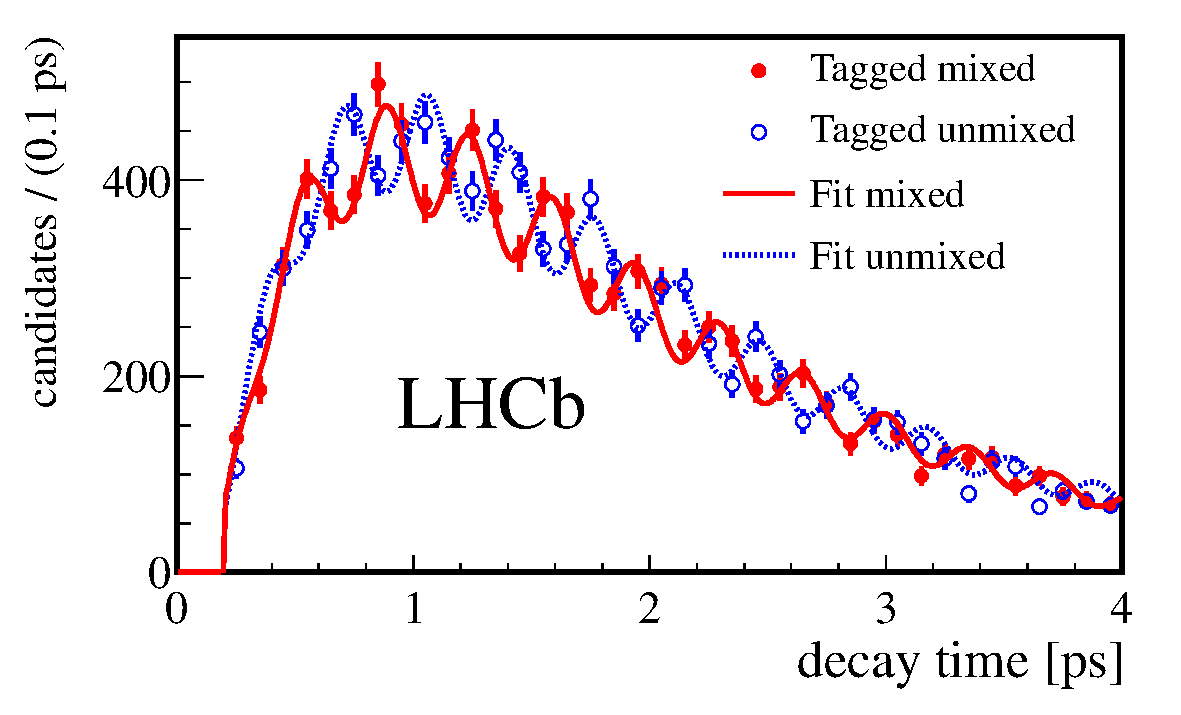
\includegraphics[height=3.5cm]{figs/lhcb/bsmix.pdf}};
          \node[draw=none,barcolor!80!black] at (2.2,0.15) {\tiny \href{http://iopscience.iop.org/1367-2630/15/5/053021/}{New~J.~Phys. 15 (2013) 053021}};
        \end{tikzpicture}
      \end{column}
      \begin{column}{0.36\textwidth}
        \begin{tikzpicture}
          \node[anchor=south west,inner sep=0] at (0,0) {\includegraphics[height=3.5cm]{figs/lhcb/RICH.png}};
          \node[draw=none,barcolor!80!black] at (1.4,0.15) {\tiny \href{http://epjc.epj.org/articles/epjc/abs/2013/05/10052_2013_Article_2431/10052_2013_Article_2431.html}{Eur. Phys. J. C (2013) 73}};
          \end{tikzpicture}
      \end{column}
    \end{columns}
\end{frame}

%%%%%%%%%%%%%%%%%%%%%%%%%%%%%%%%%%%%%%%%%%%%%%%%%%%%%%%%%%%%%%%%%
%Slide
%%%%%%%%%%%%%%%%%%%%%%%%%%%%%%%%%%%%%%%%%%%%%%%%%%%%%%%%%%%%%%%%%
\begin{frame}\frametitle{}
  \begin{center}
    \begin{tikzpicture}
      \node[anchor=south west,inner sep=0](image) at (0,0) {\includegraphics[width=\textwidth]{figs/lhcb/lhcb2.png}};
      
      \begin{scope}[x={(image.south east)},y={(image.north west)}]
        %\draw[help lines,xstep=.1,ystep=.1] (0,0) grid (1,1);
        
        \node[draw=none,burgundy] at (0.15,0.05) {Vertex Locator};
        \draw[ultra thick,->,burgundy] (0.15,0.1) -- (0.2,0.4);
        
        \node[draw=none,cadmiumorange] at (0.18,0.95) {Tracking system (TT,IT,OT)};
        \draw[ultra thick,->,cadmiumorange] (0.1,0.9) -- (0.3,0.48);
        \draw[ultra thick,->,cadmiumorange] (0.1,0.9) -- (0.58,0.52); 
        
        \node[draw=none,byzantine] at (0.48,0.95) {Rich detectors};
        \draw[ultra thick,->,byzantine] (0.5,0.9) -- (0.23,0.55);
        \draw[ultra thick,->,byzantine] (0.5,0.9) -- (0.65,0.65);
        
        \node[draw=none,gray] at (0.45,0.2) {Magnet};
        
        \node[draw=none,babyblue] at (0.7,0.05) {Calorimeters};
        \draw[ultra thick,->,babyblue] (0.7,0.1) -- (0.75,0.55);
        
        \node[draw=none,green] at (0.9,0.7) {Muon system};
        
      \end{scope}
    \end{tikzpicture}
    
  \end{center}
\end{frame}

%%%%%%%%%%%%%%%%%%%%%%%%%%%%%%%%%%%%%%%%%%%%%%%%%%%%%%%%%%%%%%%%%
%Slide
%%%%%%%%%%%%%%%%%%%%%%%%%%%%%%%%%%%%%%%%%%%%%%%%%%%%%%%%%%%%%%%%%
\begin{frame}{Track reconstruction at \lhcb}

\end{frame}

%%%%%%%%%%%%%%%%%%%%%%%%%%%%%%%%%%%%%%%%%%%%%%%%%%%%%%%%%%%%%%%%%
%Slide
%%%%%%%%%%%%%%%%%%%%%%%%%%%%%%%%%%%%%%%%%%%%%%%%%%%%%%%%%%%%%%%%%
\begin{frame}{\BdToKpimm}

\end{frame}

%%%%%%%%%%%%%%%%%%%%%%%%%%%%%%%%%%%%%%%%%%%%%%%%%%%%%%%%%%%%%%%%%
%Backup
%%%%%%%%%%%%%%%%%%%%%%%%%%%%%%%%%%%%%%%%%%%%%%%%%%%%%%%%%%%%%%%%%
\appendix

%%%%%%%%%%%%%%%%%%%%%%%%%%%%%%%%%%%%%%%%%%%%%%%%%%%%%%%%%%%%%%%%%
%Slide
%%%%%%%%%%%%%%%%%%%%%%%%%%%%%%%%%%%%%%%%%%%%%%%%%%%%%%%%%%%%%%%%%
\begin{frame}[plain]
\centering 
\Huge Backup slides
\end{frame}

%%%%%%%%%%%%%%%%%%%%%%%%%%%%%%%%%%%%%%%%%%%%%%%%%%%%%%%%%%%%%%%%%
%Slide
%%%%%%%%%%%%%%%%%%%%%%%%%%%%%%%%%%%%%%%%%%%%%%%%%%%%%%%%%%%%%%%%%
\begin{frame}{}

\end{frame}

%%%%%%%%%%%%%%%%%%%%%%%%%%%%%%%%%%%%%%%%%%%%%%%%%%%%%%%%%%%%%%%%%%%%%%%%%%%%%%%%%%%%%%%
%%%%%%%%%%%%%%%%%%%%%%%%%%%%%%%%%%%%%%%%%%%%%%%%%%%%%%%%%%%%%%%%%%%%%%%%%%%%%%%%%%%%%%%
%           END OF DOCUMENT
%%%%%%%%%%%%%%%%%%%%%%%%%%%%%%%%%%%%%%%%%%%%%%%%%%%%%%%%%%%%%%%%%%%%%%%%%%%%%%%%%%%%%%%
%%%%%%%%%%%%%%%%%%%%%%%%%%%%%%%%%%%%%%%%%%%%%%%%%%%%%%%%%%%%%%%%%%%%%%%%%%%%%%%%%%%%%%%
\end{document}


